\documentclass{beamer}


\usepackage[english]{babel}
\usepackage[utf8]{inputenc}
\usepackage{lmodern}% http://ctan.org/pkg/lm
%\usepackage{times} %font
\usepackage{amsmath, amsthm, amssymb}
\usepackage{fontawesome}

\usepackage[backend=biber, style=nature, natbib=true, date=year, sorting=ynt, doi=false,isbn=false,url=false,eprint=false, maxbibnames=1]{biblatex} 
\AtEveryBibitem{\clearfield{pages}} 
\addbibresource{references.bib}

\usetheme{Custom} % beamerThemeCustom.sty
\usepackage[orientation=portrait,size=a0,scale=1.2]{beamerposter}

\usepackage{csquotes}
\usepackage{booktabs}
\usepackage{siunitx}
\usepackage[margin=0.03\textwidth, labelformat=parens]{caption}


\title{Austrian Beekeeper Citizens Science Survey, the Financial Burden to Fight \textit{Varroa Destructor} \large{[in progress]}}
\author[\faEnvelope{} hoberreiter@gmail.com \faTwitter{} @btree\_hannes]{Hannes Oberreiter}
\institute{University Graz, Institut of Biology}
\date{\today}
\logo{\includegraphics[height=5.5cm]{img/logo_uni_graz_4c.jpg}}

\begin{document}

\begin{frame}{} 

\begin{columns}[t]
  \begin{column}{0.49\textwidth}

    \begin{block}{Introduction}
      My master thesis deals with beekeeping in Austria and the expenses involved in the use of medication against the parasitic mite \textit{Varroa destructor}. In the foreground of the work is an exploratory analysis of citizen science survey data from the years 2018/19 and 2019/20 which is done yearly in Austria since 2008 by the University of Graz \citep{brodschneider2013}.
      \\
      \begin{figure}
        \centering
        \includegraphics[width=.5\textwidth]{img/drawing.png}
      \end{figure}
      \setlength{\leftmargini}{95pt}
      \begin{itemize}
        \setlength{\itemindent}{-30pt}
        \LARGE
          \item Analysis of the economic burden of beekeepers to fight the introduced aggressor \textit{Varroa destructor}
          \item Dimensions of the Austrian treatment agent market
          \item Hypothesis about loss and expenses correlation of different treatment methods
      \end{itemize}
      \vspace{39pt}
    \end{block}

    \begin{block}{Material and Methods}
      The survey consisted of questions from the international COLOSS questionnaire \citep{vanderzee2013} and some additional questions which were only present in the Austrian survey.
        
      \setlength{\leftmargini}{95pt}
      \begin{itemize}
        \setlength{\itemindent}{-30pt}
        \LARGE
          \item Data of two years and more than 2.000 responses
          \item Open source and fully reproducible code as goal
      \end{itemize}
    
      \begin{figure} 
        \centering
        \includegraphics[width=.85\textwidth]{img/map.pdf}
        \caption{The approximate location of the main winter apiary showed a nationwide coverage all over Austria for both survey years. Shapefiles, \enquote{Creative Commons}: \url{https://www.data.gv.at/}}
      \end{figure}
      
            \hrulefill
      \vspace{15pt}
      \begin{table}
        \centering
        \caption{Descriptive statistics of expenses per colony in comparison to our own estimation of expenses, in Euro. Both survey years together.}
        \begin{tabular}[]{l*{6}{S[table-format=4.4]}}
          \toprule
          Type & {Minimum} & {1. Quantile} & {Median} & {Mean} & {3. Quantile} & {Maximum}\tabularnewline
          \midrule
          Survey & 0.00 & 5.00 & 8.33 & 9.98 & 12.50 & 250.00 \tabularnewline
          Estimated & 0.00 & 8.05 & 10.65 & 12.18 & 14.02 & 167.32 \tabularnewline
          \bottomrule
        \end{tabular}
      \end{table}
      \vspace{15pt}
      
    \end{block}
    
    {
      \setbeamercolor*{block title}{fg=taaluminium,bg=ta3chameleon}
      \begin{block}{Preemptive Conclusion}
         \setlength{\leftmargini}{95pt}
          \begin{itemize}
          \setlength{\itemindent}{-30pt}
          \LARGE
          \item Calculated estimates are in line with survey
          \item Significant lower expenses per colony for bigger beekeeping operations
          \item Further analysis in progress
        \end{itemize}
      \end{block}
    }

  \end{column}

  \begin{column}{0.49\textwidth}  
    {
      \setbeamercolor*{block title}{fg=taaluminium,bg=ta3skyblue}
      \begin{block}{Info Box - Varroa Mite}
      \setlength{\leftmargini}{95pt}
        \begin{itemize}
            \setlength{\itemindent}{-30pt}
            \item Most important honeybee pest worldwide, in Austria since the 1980s
            \item Mainly in the brood and there preferable in the drone brood \citep{rosenkranz2010}
            \item Feeds primarily on the fat body of larvae and adult bees, which are also used as phoretic transport medium \citep{ramsey2019}
            \item Great influence on the overwintering success of bee colonies \citep{dahle2010}
            \item Vector for other pathogens, such as viruses \citep{rosenkranz2010, noel2020}
            \item In Austria most beekeepers use a combination of organic acids to treat their colonies against the Varroa mite \citep{moosbeckhofer2015, oberreiter2020}
        \end{itemize}

        \begin{figure}
          \centering
          \includegraphics[height=400pt]{img/varroa.jpg}
          \includegraphics[height=400pt]{img/mite_inat.jpg}
          \caption{Image of Varroa mites infested drone brood and microscope picture of an adult female (2mm wide bar below). Photo © Hannes Oberreiter (left), dava123 from iNaturalist.org (right)}
        \end{figure}

      \end{block}
    }
    
    \begin{block}{Preemptive Results}
      \begin{figure}
        \centering
        \includegraphics[width=0.8\textwidth]{img/distr-year-1.pdf}
        \caption{Distribution of expenses as violin plot in combination with a boxplot. Maximum values are cutoff.}
      \end{figure}

      \hrulefill
      \vspace{0pt}

      \begin{figure}
        \centering
        \includegraphics[width=0.8\textwidth]{img/operation.pdf}
        \caption{To compare different operation size groups, we used the number of colonies wintered from the survey to group the beekeepers in their respective operation size groups. Stars indicating statistically significant difference.}
      \end{figure}
    \end{block}
    
    {
        \vspace{10pt}
        \vskip.75ex
        \setbeamercolor{ref}{fg=white,bg=black}
        \begin{beamercolorbox}[rounded=false,shadow=false,colsep*=.75ex,sep=.75ex,vmode]{ref}
          \par\leftskip=20pt\rightskip=20pt
            \small{References:}
            \footnotesize
            \printbibliography
        \end{beamercolorbox}
    }
  
  \end{column}
\end{columns}

\vfill
\end{frame}
\end{document}